% last update november 2019
\documentclass{esannV2}
\usepackage{graphicx}
%\usepackage[latin1]{inputenc}
\usepackage{amssymb,amsmath,array}
\usepackage[utf8]{inputenc}   % Soporte para caracteres UTF-8
\usepackage[spanish]{babel}   % Configuración del idioma español


\usepackage{booktabs}


%***********************************************************************
% !!!! IMPORTANT NOTICE ON TEXT MARGINS !!!!!
%***********************************************************************
%
% Please avoid using DVI2PDF or PS2PDF converters: some undesired
% shifting/scaling may occur when using these programs
% It is strongly recommended to use the DVIPS converters, and to submit
% PS file. You may submit a PDF file if and only if you use ADOBE ACROBAT
% to convert your PS file to PDF.
%
% Check that you have set the paper size to A4 (and NOT to letter) in your
% dvi2ps converter, in Adobe Acrobat if you use it, and in any printer driver
% that you could use.  You also have to disable the 'scale to fit paper' option
% of your printer driver.
%
% In any case, please check carefully that the final size of the top and
% bottom margins is 5.2 cm and of the left and right margins is 4.4 cm.
% It is your responsibility to verify this important requirement.  If these margin requirements and not fulfilled at the end of your file generation process, please use the following commands to correct them.  Otherwise, please do not modify these commands.
%
\voffset 0 cm \hoffset 0 cm \addtolength{\textwidth}{0cm}
\addtolength{\textheight}{0cm}\addtolength{\leftmargin}{0cm}

%***********************************************************************
% !!!! USE OF THE esannV2 LaTeX STYLE FILE !!!!!
%***********************************************************************
%
% Some commands are inserted in the following .tex example file.  Therefore to
% set up your ESANN submission, please use this file and modify it to insert
% your text, rather than staring from a blank .tex file.  In this way, you will
% have the commands inserted in the right place.

\begin{document}
%style file for ESANN manuscripts
\title{Reconocimiento de Actividades Humanas Utilizando Teléfonos Inteligentes}

%***********************************************************************
% AUTHORS INFORMATION AREA
%***********************************************************************
\author{Salgado López Álvaro$^1$
%
% Optional short acknowledgment: remove next line if non-needed
%
% DO NOT MODIFY THE FOLLOWING '\vspace' ARGUMENT
\vspace{.3cm}\\
%
% Addresses and institutions (remove "1- " in case of a single institution)
UANL - Facultad De Ciencias Físico Matemáticas \\
Av. Universidad s/n. Ciudad Universitaria San Nicolás de los Garza - México
}
%
% Remove the next three lines in case of a single institution
%***********************************************************************
% END OF AUTHORS INFORMATION AREA
%***********************************************************************
\maketitle


\section{Introducción}

El Reconocimiento de Actividades Humanas (HAR, por sus siglas en inglés) constituye un esfuerzo fundamental en el ámbito de comprender el comportamiento humano a través de medios tecnológicos. Su objetivo fundamental radica en identificar las acciones realizadas por individuos basándose en una colección de observaciones derivadas tanto del individuo como de su entorno circundante. Tradicionalmente, las metodologías de reconocimiento han aprovechado diversas fuentes de datos, que van desde señales ambientales hasta sensores colocados en el cuerpo, para lograr este objetivo. Destacadamente, los sensores de movimiento especializados ubicados en varias partes del cuerpo, como la cintura, la muñeca, el pecho y los muslos, han demostrado un rendimiento de clasificación notable. Sin embargo, estas configuraciones de sensores convencionales a menudo conllevan incomodidad para los usuarios y no ofrecen una solución sostenible a largo plazo para el monitoreo de actividades.

El advenimiento de los teléfonos inteligentes ha inaugurado una nueva era de oportunidades de investigación en aplicaciones centradas en el ser humano. Con los usuarios como fuentes de información contextual y los teléfonos inteligentes como herramientas de detección primarias, estos dispositivos ubicuos equipados con una variedad de sensores integrados, incluidos acelerómetros, giroscopios, micrófonos y cámaras duales, presentan una alternativa atractiva para el HAR. Al aprovechar los sensores inerciales incorporados en los teléfonos inteligentes, los investigadores han comenzado a explorar vías para monitorear automáticamente y de manera discreta las Actividades de la Vida Diaria (AVD). Notablemente, los teléfonos inteligentes brindan una solución flexible, asequible y autónoma que integra perfectamente el monitoreo de actividades con servicios de telefonía \cite{esann2013}.

En este trabajo, se exploran técnicas de aprendizaje no supervisado para clasificar diferentes tipos de actividades físicas a partir de datos recogidos por sensores. A diferencia de los métodos supervisados, los algoritmos no supervisados no requieren un conjunto de datos previamente etiquetados para entrenar el modelo, lo cual puede ser ventajoso en escenarios donde la obtención de datos etiquetados es costosa o impráctica.

\section{Metodología}
Se llevaron a cabo una serie de experimentos para obtener el conjunto de datos HAR. Se seleccionó un grupo de 30 voluntarios con edades comprendidas entre los 19 y 48 años para esta tarea. A cada persona se le indicó seguir un protocolo de actividades mientras llevaba un teléfono inteligente Samsung Galaxy S II montado en la cintura. Las seis actividades de la vida diaria (ADL) seleccionadas fueron estar de pie, sentarse, acostarse, caminar, bajar escaleras y subir escaleras. Cada sujeto realizó el protocolo dos veces: en el primer intento, el teléfono inteligente se colocó en el lado izquierdo del cinturón, y en el segundo, el usuario mismo lo colocó según su preferencia. También hubo una separación de 5 segundos entre cada tarea, donde se les indicaba a los individuos descansar, lo que facilitó la repetibilidad (cada actividad se intentó al menos dos veces) y la generación de datos de referencia a través de la interfaz visual.

\begin{table}[h!]
    \centering
    \resizebox{\textwidth}{!}{%
    \begin{tabular}{|c|l|c|c|l|c|}
        \hline
        \textbf{No.} & \textbf{Estático} & \textbf{Tiempo (seg)} & \textbf{No.} & \textbf{Dinámico} & \textbf{Tiempo (seg)} \\
        \hline
        0 & Inicio (De pie Pos) & 0 & 7 & Caminar (1) & 15 \\
        1 & De pie (1) & 15 & 8 & Caminar (2) & 15 \\
        2 & Sentarse (1) & 15 & 9 & Bajar escaleras (1) & 12 \\
        3 & De pie (2) & 15 & 10 & Subir escaleras (2) & 12 \\
        4 & Acostarse (1) & 15 & 11 & Bajar escaleras (1) & 12 \\
        5 & Sentarse (2) & 15 & 12 & Subir escaleras (2) & 12 \\
        6 & Acostarse (2) & 15 & 13 & Bajar escaleras (3) & 12 \\

        & & & 14 & Subir escaleras (3) & 12 \\
        & & & 15 & Detenerse & 0 \\
        \hline
        \multicolumn{5}{|r|}{\textbf{Total}} & \textbf{192} \\
        \hline
    \end{tabular}
    }
    \caption{Protocolo de actividades para el Experimento HAR.}
    \label{tab:har_protocol}
\end{table}

Las tareas se realizaron en condiciones de laboratorio, pero se les pidió a los voluntarios que realizaran libremente la secuencia de actividades para obtener un conjunto de datos más naturalista. El Cuadro 1 muestra los detalles del protocolo experimental \cite{esann2013}.

\subsection{Aprendizaje no supervisado}
Además del popular algoritmo de aprendizaje no supervisado K-Means, una alternativa poderosa para abordar el reconocimiento de actividades humanas (HAR) en conjuntos de datos complejos es el modelo de mezclas gaussianas (GMM, por sus siglas en inglés).

El algoritmo de GMM es especialmente eficaz cuando se trabaja con datos que poseen características continuas, como aquellas obtenidas de sensores de acelerómetro y giroscopio. A diferencia de K-Means, que asigna cada punto de datos a un solo clúster, GMM modela la distribución de los datos como una mezcla de varias distribuciones gaussianas. Esto significa que GMM puede capturar la complejidad de conjuntos de datos donde los puntos pueden pertenecer a múltiples clústeres o grupos.

Un GMM asume que los datos son generados a partir de una combinación (mezcla) de varias distribuciones gaussianas (normales), cada una con su propia media y varianza. Matemáticamente, esto se expresa como:

\begin{eqnarray}
p(x) = \sum_{k=1}^{K} \pi_{k} \mathcal{N}(x | \mu_{k}, \Sigma_{k})
\end{eqnarray}
Donde:

$\mathcal{N}(x | \mu_{k}, \Sigma_{k})$ es una distribución gaussiana con media $\mu_{k}$ y covarianza $\Sigma_{k}$.


$\pi_{k}$ es el peso de la k-ésima componente gaussiana (con $\sum_{k=1}^{K} \pi_{k} = 1$).

%t is your responsibility to verify this important requirement.  If these margin requirements and not fulfilled at the end of your file generation process, please use the commands at the beginning of the ESANNV2.tex file to correct them.  Otherwise, please do not modify these commands.

\subsection{Aprendizaje supervisado}
Se optó por utilizar el algoritmo de Máquinas de Vectores de Soporte (SVM, por sus siglas en inglés) debido a su eficacia en espacios de alta dimensión, lo cual es ideal para este conjunto de datos ya que contiene características extraídas de múltiples sensores de teléfonos inteligentes, como acelerómetros y giroscopios. Las características en este conjunto de datos pueden ser complejas y altamente dimensionales, y SVM puede encontrar un hiperplano óptimo que separa eficazmente las diferentes actividades humanas en este espacio de características. Además, algunas variantes de SVM han demostrado previamente su capacidad en problemas similares, obteniendo buenos resultados \cite{anguitaSVM}.

SVM utiliza una función de pérdida hinge para maximizar el margen y minimizar el error de clasificación:
\[
\min_{\mathbf{w}, b} \frac{1}{2} \| \mathbf{w} \|^2 + C \sum_{i=1}^n \max(0, 1 - y_i (\mathbf{w} \cdot \mathbf{x}_i + b)),
\]
donde \( \| \mathbf{w} \|^2 \) es la norma cuadrada del vector de pesos \( \mathbf{w} \), \( C \) es el parámetro de regularización que controla el trade-off entre el margen y el error de clasificación, \( \mathbf{x}_i \) son las muestras de entrenamiento, y \( y_i \) son las etiquetas de clase correspondientes (\( y_i \in \{-1, 1\} \)).


\section{Resultados}
\subsection{Aprendizaje no supervisado}
Luego de implementar el algoritmo de GGM se obtuvo una clasificación de las actividades realizadas.
\begin{figure}[ht!]
\centering
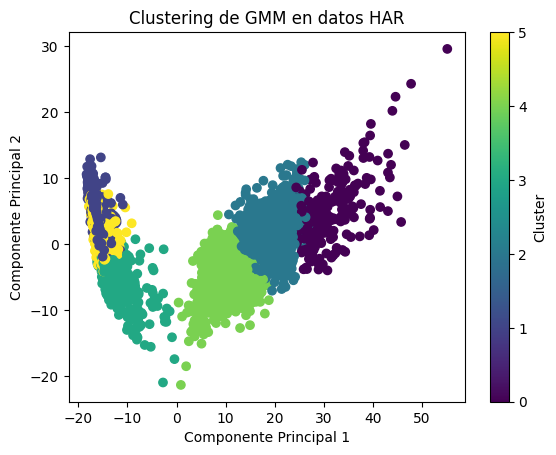
\includegraphics[width=0.5\textwidth]{figs/Resultados.png}
\caption{Clustering de GMM en datos HAR}\label{Fig:resultados}
\end{figure}
Se empleó el algoritmo de GMM para abordar la clasificación de las HAR. Los resultados de esta aplicación se presentan en la Figura 1.

Los hallazgos revelan una exitosa clasificación, donde se muestran claramente 6 grupos distintos en la Figura, cada uno representado con un color único. Cabe destacar que cada uno de estos grupos corresponde a una de las 6 actividades realizadas durante el estudio.

Este enfoque de clasificación basado en GMM permite una visualización clara y una interpretación precisa de los patrones de actividad identificados en los datos de HAR. La capacidad del algoritmo para modelar distribuciones complejas de datos y asignar probabilidades de pertenencia a múltiples clústeres ha demostrado ser efectiva en la identificación de diferentes actividades humanas, incluso en casos donde existen superposiciones o variaciones sutiles entre las actividades.

\subsection{Aprendizaje Supervisado}
Tras la implementación del algoritmo SVM, se logró alcanzar una precisión del 98\%. Este resultado refleja que el modelo pudo clasificar correctamente un alto porcentaje de los datos del conjunto de prueba, demostrando su eficacia en la tarea de reconocimiento de actividades humanas basadas en datos de sensores de teléfonos inteligentes. La alta precisión obtenida demuestra la capacidad del SVM para manejar de manera efectiva las características complejas y multidimensionales extraídas de los sensores, como acelerómetros y giroscopios.
\begin{figure}[ht!]
\centering
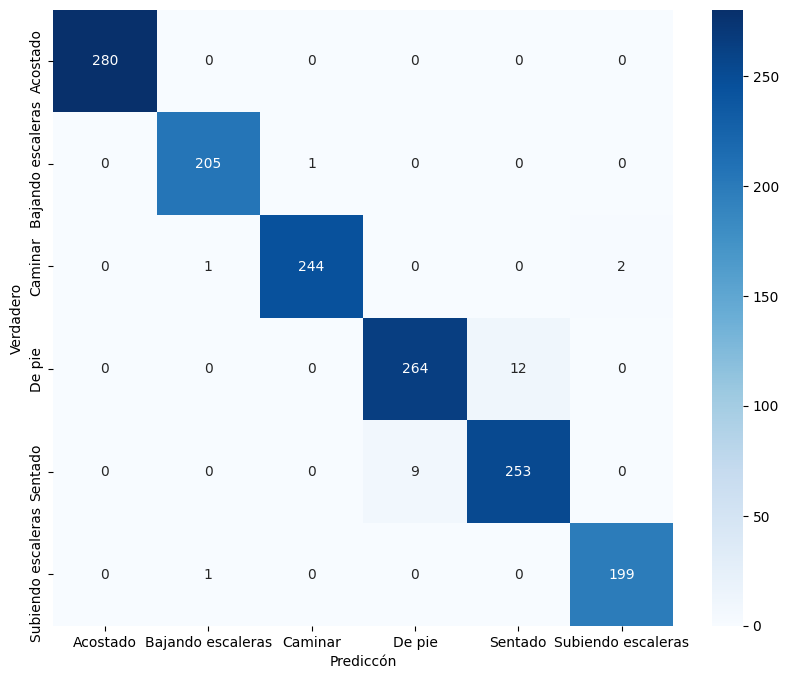
\includegraphics[width=0.5\textwidth]{figs/SVM_matriz.png}
\caption{Matriz de Confusión}\label{Fig:matriz_SVG}
\end{figure}
Además, la Figura 2 presenta detalladamente la matriz de confusión generada por el modelo. Esta matriz proporciona de manera visual cómo se clasificaron las diferentes actividades, mostrando el número de predicciones correctas e incorrectas para cada clase. Por ejemplo, se observa que la mayoría de las actividades fueron clasificadas con precisión casi perfecta.

El reporte de clasificación también destaca la sensibilidad (recall) del modelo de 98\%, que indica la capacidad del SVM para identificar correctamente las muestras de cada clase. En general, el modelo mostró una alta sensibilidad en todas las actividades, lo que refuerza su robustez y confiabilidad en aplicaciones prácticas.


\section{Conclusión}
En este estudio, se exploró el uso del algoritmo de Gaussian Mixture Models (GMM) para clasificar las Actividades Humanas Reconocidas (HAR). El conjunto de datos utilizado en este estudio contiene el etiquetado de las actividades, lo que permitió una evaluación directa del desempeño del algoritmo sin necesidad de calcular el número de grupos.

Mediante el análisis de los resultados obtenidos, se ha demostrado la eficacia de GMM en la clasificación precisa de actividades humanas basadas en datos de sensores de acelerómetro y giroscopio. Los hallazgos revelaron que GMM es capaz de identificar patrones complejos en los datos de HAR y asignar de manera efectiva las observaciones a diferentes clústeres que representan actividades específicas. La capacidad de GMM para modelar la distribución de los datos de manera flexible y capturar las relaciones no lineales entre las características contribuyó significativamente a su rendimiento en la clasificación de actividades humanas.

Además, se observó que GMM proporciona una visualización clara de las actividades identificadas, lo que facilita la interpretación de los resultados y la identificación de patrones significativos. Esta capacidad de interpretación es crucial para aplicaciones prácticas en áreas como el monitoreo de la salud, la rehabilitación física y la optimización del rendimiento deportivo.

Adicionalente, el SVM se presenta como una solución eficaz y confiable para el reconocimiento de actividades humanas, ofreciendo un alto nivel de precisión y capacidad para gestionar múltiples clases de actividades de manera efectiva. Estos resultados son prometedores para su implementación en sistemas de seguimiento y análisis de actividades diarias, proporcionando una solución robusta y precisa para el monitoreo basado en datos de sensores.


% ****************************************************************************
% BIBLIOGRAPHY AREA
% ****************************************************************************

\begin{footnotesize}

% IF YOU DO NOT USE BIBTEX, USE THE FOLLOWING SAMPLE SCHEME FOR THE REFERENCES
% ----------------------------------------------------------------------------

\bibliographystyle{IEEEtran}
\bibliography{referencias}



% ----------------------------------------------------------------------------

% IF YOU USE BIBTEX,
% - DELETE THE TEXT BETWEEN THE TWO ABOVE DASHED LINES
% - UNCOMMENT THE NEXT TWO LINES AND REPLACE 'Name_Of_Your_BibFile'

%\bibliographystyle{unsrt}
%\bibliography{Name_Of_Your_BibFile}

\end{footnotesize}

% ****************************************************************************
% END OF BIBLIOGRAPHY AREA
% ****************************************************************************

\end{document}
